%%%%%%%%%%%%%%%%%%%%%%%%%%%%%%%%%%%%%%%%%%%%%%%%%%%%%%%%%%%%%%%%%%%%%%%%
% Escuela Politécnica Superior de la Universidad de Alicante
% Realizado por: Jose Manuel Requena Plens
% Contacto: info@jmrplens.com / Telegram:@jmrplens
%%%%%%%%%%%%%%%%%%%%%%%%%%%%%%%%%%%%%%%%%%%%%%%%%%%%%%%%%%%%%%%%%%%%%%%%

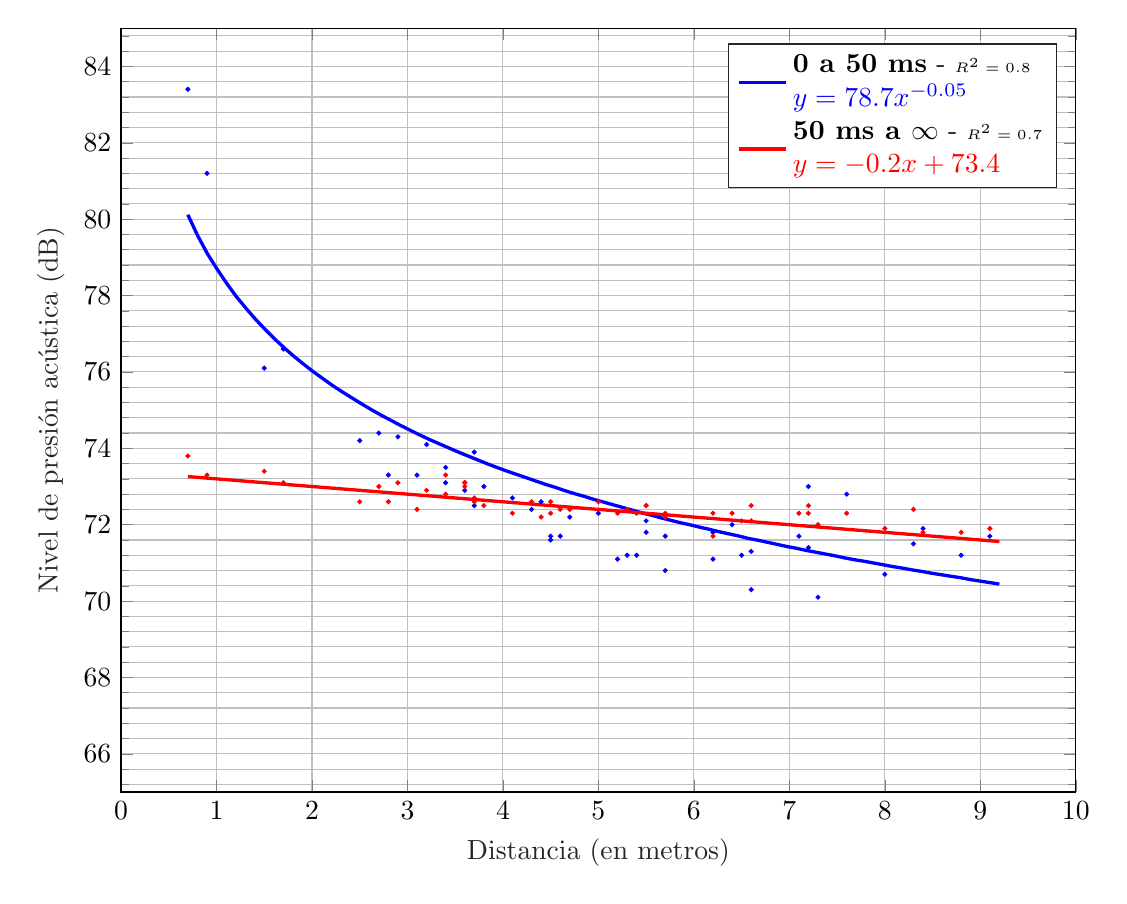
\begin{tikzpicture}

\begin{axis}[%
width=\textwidth,
height=0.8\textwidth,
at={(0\textwidth,0\textwidth)},
scale only axis,
xmin=0,
xmax=10,
xlabel style={font=\color{white!15!black}},
xlabel={Distancia (en metros)},
ymin=65,
ymax=85,
xmajorgrids,
xminorgrids,
ymajorgrids,
yminorgrids,
minor y tick num= 4,
ylabel style={font=\color{white!15!black}},
ylabel={Nivel de presión acústica (dB)},
axis background/.style={fill=white},
%xmajorgrids,
%xminorgrids,
%ymajorgrids,
%yminorgrids,
legend style={legend cell align=left, align=left, draw=white!15!black}
]
\addplot[color=blue,domain=0.7:9.2, samples=85,line width=1.2]{78.7*x^(-0.05)};
\addlegendentry{\textbf{0 a 50 ms} - \tiny{$R^2 = 0.8$}\\$\color{blue}y = 78.7·x^{-0.05}$}

\addplot[color=red,domain=0.7:9.2, samples=85,line width=1.2]{-0.2*x+73.40};
\addlegendentry{\textbf{50 ms a $\infty$} - \tiny{$R^2 = 0.7$}\\$\color{red}y = -0.2·x+73.4$}

% Puntos
\addplot [color=blue, only marks,mark size=0.7pt]
  table[row sep=crcr]{%
  9.1	71.7\\
8.3	71.5\\
7.2	71.4\\
6.4	72.0\\
5.5	72.1\\
4.7	72.2\\
4.1	72.7\\
3.6	73.1\\
3.4	73.5\\
3.4	73.1\\
3.7	72.5\\
4.3	72.4\\
5.0	72.3\\
5.7	71.7\\
6.5	71.2\\
7.3	70.1\\
8.4	71.9\\
5.2	71.1\\
6.6	71.3\\
5.5	71.8\\
4.5	71.6\\
7.6	72.8\\
2.5	74.2\\
1.5	76.1\\
0.7	83.4\\
0.9	81.2\\
1.7	76.6\\
2.7	74.4\\
3.6	72.9\\
4.6	71.7\\
5.7	70.8\\
6.6	70.3\\
8.8	71.2\\
8.0	70.7\\
7.1	71.7\\
6.2	71.8\\
5.3	71.2\\
4.4	72.6\\
3.7	73.9\\
3.1	73.3\\
2.8	73.3\\
2.9	74.3\\
3.2	74.1\\
3.8	73.0\\
4.5	71.7\\
5.4	71.2\\
6.2	71.1\\
7.2	73.0\\
  };
  
  \addplot [color=red, only marks,mark size=0.7pt]
  table[row sep=crcr]{%
  9.1	71.9\\
8.3	72.4\\
7.2	72.3\\
6.4	72.3\\
5.5	72.5\\
4.7	72.4\\
4.1	72.3\\
3.6	73.0\\
3.4	73.3\\
3.4	72.8\\
3.7	72.6\\
4.3	72.6\\
5.0	72.6\\
5.7	72.2\\
6.5	72.1\\
7.3	72.0\\
8.4	71.8\\
5.2	72.3\\
6.6	72.1\\
5.5	72.5\\
4.5	72.3\\
7.6	72.3\\
2.5	72.6\\
1.5	73.4\\
0.7	73.8\\
0.9	73.3\\
1.7	73.1\\
2.7	73.0\\
3.6	73.1\\
4.6	72.4\\
5.7	72.3\\
6.6	72.5\\
8.8	71.8\\
8.0	71.9\\
7.1	72.3\\
6.2	71.7\\
5.3	72.4\\
4.4	72.2\\
3.7	72.7\\
3.1	72.4\\
2.8	72.6\\
2.9	73.1\\
3.2	72.9\\
3.8	72.5\\
4.5	72.6\\
5.4	72.3\\
6.2	72.3\\
7.2	72.5\\
  };
\end{axis}
\end{tikzpicture}%